% Options for packages loaded elsewhere
\PassOptionsToPackage{unicode}{hyperref}
\PassOptionsToPackage{hyphens}{url}
\PassOptionsToPackage{dvipsnames,svgnames,x11names}{xcolor}
%
\documentclass[
  letterpaper,
  DIV=11,
  numbers=noendperiod]{scrreprt}

\usepackage{amsmath,amssymb}
\usepackage{iftex}
\ifPDFTeX
  \usepackage[T1]{fontenc}
  \usepackage[utf8]{inputenc}
  \usepackage{textcomp} % provide euro and other symbols
\else % if luatex or xetex
  \usepackage{unicode-math}
  \defaultfontfeatures{Scale=MatchLowercase}
  \defaultfontfeatures[\rmfamily]{Ligatures=TeX,Scale=1}
\fi
\usepackage{lmodern}
\ifPDFTeX\else  
    % xetex/luatex font selection
\fi
% Use upquote if available, for straight quotes in verbatim environments
\IfFileExists{upquote.sty}{\usepackage{upquote}}{}
\IfFileExists{microtype.sty}{% use microtype if available
  \usepackage[]{microtype}
  \UseMicrotypeSet[protrusion]{basicmath} % disable protrusion for tt fonts
}{}
\makeatletter
\@ifundefined{KOMAClassName}{% if non-KOMA class
  \IfFileExists{parskip.sty}{%
    \usepackage{parskip}
  }{% else
    \setlength{\parindent}{0pt}
    \setlength{\parskip}{6pt plus 2pt minus 1pt}}
}{% if KOMA class
  \KOMAoptions{parskip=half}}
\makeatother
\usepackage{xcolor}
\setlength{\emergencystretch}{3em} % prevent overfull lines
\setcounter{secnumdepth}{5}
% Make \paragraph and \subparagraph free-standing
\ifx\paragraph\undefined\else
  \let\oldparagraph\paragraph
  \renewcommand{\paragraph}[1]{\oldparagraph{#1}\mbox{}}
\fi
\ifx\subparagraph\undefined\else
  \let\oldsubparagraph\subparagraph
  \renewcommand{\subparagraph}[1]{\oldsubparagraph{#1}\mbox{}}
\fi

\usepackage{color}
\usepackage{fancyvrb}
\newcommand{\VerbBar}{|}
\newcommand{\VERB}{\Verb[commandchars=\\\{\}]}
\DefineVerbatimEnvironment{Highlighting}{Verbatim}{commandchars=\\\{\}}
% Add ',fontsize=\small' for more characters per line
\usepackage{framed}
\definecolor{shadecolor}{RGB}{241,243,245}
\newenvironment{Shaded}{\begin{snugshade}}{\end{snugshade}}
\newcommand{\AlertTok}[1]{\textcolor[rgb]{0.68,0.00,0.00}{#1}}
\newcommand{\AnnotationTok}[1]{\textcolor[rgb]{0.37,0.37,0.37}{#1}}
\newcommand{\AttributeTok}[1]{\textcolor[rgb]{0.40,0.45,0.13}{#1}}
\newcommand{\BaseNTok}[1]{\textcolor[rgb]{0.68,0.00,0.00}{#1}}
\newcommand{\BuiltInTok}[1]{\textcolor[rgb]{0.00,0.23,0.31}{#1}}
\newcommand{\CharTok}[1]{\textcolor[rgb]{0.13,0.47,0.30}{#1}}
\newcommand{\CommentTok}[1]{\textcolor[rgb]{0.37,0.37,0.37}{#1}}
\newcommand{\CommentVarTok}[1]{\textcolor[rgb]{0.37,0.37,0.37}{\textit{#1}}}
\newcommand{\ConstantTok}[1]{\textcolor[rgb]{0.56,0.35,0.01}{#1}}
\newcommand{\ControlFlowTok}[1]{\textcolor[rgb]{0.00,0.23,0.31}{#1}}
\newcommand{\DataTypeTok}[1]{\textcolor[rgb]{0.68,0.00,0.00}{#1}}
\newcommand{\DecValTok}[1]{\textcolor[rgb]{0.68,0.00,0.00}{#1}}
\newcommand{\DocumentationTok}[1]{\textcolor[rgb]{0.37,0.37,0.37}{\textit{#1}}}
\newcommand{\ErrorTok}[1]{\textcolor[rgb]{0.68,0.00,0.00}{#1}}
\newcommand{\ExtensionTok}[1]{\textcolor[rgb]{0.00,0.23,0.31}{#1}}
\newcommand{\FloatTok}[1]{\textcolor[rgb]{0.68,0.00,0.00}{#1}}
\newcommand{\FunctionTok}[1]{\textcolor[rgb]{0.28,0.35,0.67}{#1}}
\newcommand{\ImportTok}[1]{\textcolor[rgb]{0.00,0.46,0.62}{#1}}
\newcommand{\InformationTok}[1]{\textcolor[rgb]{0.37,0.37,0.37}{#1}}
\newcommand{\KeywordTok}[1]{\textcolor[rgb]{0.00,0.23,0.31}{#1}}
\newcommand{\NormalTok}[1]{\textcolor[rgb]{0.00,0.23,0.31}{#1}}
\newcommand{\OperatorTok}[1]{\textcolor[rgb]{0.37,0.37,0.37}{#1}}
\newcommand{\OtherTok}[1]{\textcolor[rgb]{0.00,0.23,0.31}{#1}}
\newcommand{\PreprocessorTok}[1]{\textcolor[rgb]{0.68,0.00,0.00}{#1}}
\newcommand{\RegionMarkerTok}[1]{\textcolor[rgb]{0.00,0.23,0.31}{#1}}
\newcommand{\SpecialCharTok}[1]{\textcolor[rgb]{0.37,0.37,0.37}{#1}}
\newcommand{\SpecialStringTok}[1]{\textcolor[rgb]{0.13,0.47,0.30}{#1}}
\newcommand{\StringTok}[1]{\textcolor[rgb]{0.13,0.47,0.30}{#1}}
\newcommand{\VariableTok}[1]{\textcolor[rgb]{0.07,0.07,0.07}{#1}}
\newcommand{\VerbatimStringTok}[1]{\textcolor[rgb]{0.13,0.47,0.30}{#1}}
\newcommand{\WarningTok}[1]{\textcolor[rgb]{0.37,0.37,0.37}{\textit{#1}}}

\providecommand{\tightlist}{%
  \setlength{\itemsep}{0pt}\setlength{\parskip}{0pt}}\usepackage{longtable,booktabs,array}
\usepackage{calc} % for calculating minipage widths
% Correct order of tables after \paragraph or \subparagraph
\usepackage{etoolbox}
\makeatletter
\patchcmd\longtable{\par}{\if@noskipsec\mbox{}\fi\par}{}{}
\makeatother
% Allow footnotes in longtable head/foot
\IfFileExists{footnotehyper.sty}{\usepackage{footnotehyper}}{\usepackage{footnote}}
\makesavenoteenv{longtable}
\usepackage{graphicx}
\makeatletter
\def\maxwidth{\ifdim\Gin@nat@width>\linewidth\linewidth\else\Gin@nat@width\fi}
\def\maxheight{\ifdim\Gin@nat@height>\textheight\textheight\else\Gin@nat@height\fi}
\makeatother
% Scale images if necessary, so that they will not overflow the page
% margins by default, and it is still possible to overwrite the defaults
% using explicit options in \includegraphics[width, height, ...]{}
\setkeys{Gin}{width=\maxwidth,height=\maxheight,keepaspectratio}
% Set default figure placement to htbp
\makeatletter
\def\fps@figure{htbp}
\makeatother
\newlength{\cslhangindent}
\setlength{\cslhangindent}{1.5em}
\newlength{\csllabelwidth}
\setlength{\csllabelwidth}{3em}
\newlength{\cslentryspacingunit} % times entry-spacing
\setlength{\cslentryspacingunit}{\parskip}
\newenvironment{CSLReferences}[2] % #1 hanging-ident, #2 entry spacing
 {% don't indent paragraphs
  \setlength{\parindent}{0pt}
  % turn on hanging indent if param 1 is 1
  \ifodd #1
  \let\oldpar\par
  \def\par{\hangindent=\cslhangindent\oldpar}
  \fi
  % set entry spacing
  \setlength{\parskip}{#2\cslentryspacingunit}
 }%
 {}
\usepackage{calc}
\newcommand{\CSLBlock}[1]{#1\hfill\break}
\newcommand{\CSLLeftMargin}[1]{\parbox[t]{\csllabelwidth}{#1}}
\newcommand{\CSLRightInline}[1]{\parbox[t]{\linewidth - \csllabelwidth}{#1}\break}
\newcommand{\CSLIndent}[1]{\hspace{\cslhangindent}#1}

\usepackage{booktabs}
\usepackage{longtable}
\usepackage{array}
\usepackage{multirow}
\usepackage{wrapfig}
\usepackage{float}
\usepackage{colortbl}
\usepackage{pdflscape}
\usepackage{tabu}
\usepackage{threeparttable}
\usepackage{threeparttablex}
\usepackage[normalem]{ulem}
\usepackage{makecell}
\usepackage{xcolor}
\KOMAoption{captions}{tableheading}
\makeatletter
\makeatother
\makeatletter
\@ifpackageloaded{bookmark}{}{\usepackage{bookmark}}
\makeatother
\makeatletter
\@ifpackageloaded{caption}{}{\usepackage{caption}}
\AtBeginDocument{%
\ifdefined\contentsname
  \renewcommand*\contentsname{Tabla de contenidos}
\else
  \newcommand\contentsname{Tabla de contenidos}
\fi
\ifdefined\listfigurename
  \renewcommand*\listfigurename{Listado de Figuras}
\else
  \newcommand\listfigurename{Listado de Figuras}
\fi
\ifdefined\listtablename
  \renewcommand*\listtablename{Listado de Tablas}
\else
  \newcommand\listtablename{Listado de Tablas}
\fi
\ifdefined\figurename
  \renewcommand*\figurename{Figura}
\else
  \newcommand\figurename{Figura}
\fi
\ifdefined\tablename
  \renewcommand*\tablename{Tabla}
\else
  \newcommand\tablename{Tabla}
\fi
}
\@ifpackageloaded{float}{}{\usepackage{float}}
\floatstyle{ruled}
\@ifundefined{c@chapter}{\newfloat{codelisting}{h}{lop}}{\newfloat{codelisting}{h}{lop}[chapter]}
\floatname{codelisting}{Listado}
\newcommand*\listoflistings{\listof{codelisting}{Listado de Listados}}
\makeatother
\makeatletter
\@ifpackageloaded{caption}{}{\usepackage{caption}}
\@ifpackageloaded{subcaption}{}{\usepackage{subcaption}}
\makeatother
\makeatletter
\@ifpackageloaded{tcolorbox}{}{\usepackage[skins,breakable]{tcolorbox}}
\makeatother
\makeatletter
\@ifundefined{shadecolor}{\definecolor{shadecolor}{rgb}{.97, .97, .97}}
\makeatother
\makeatletter
\makeatother
\makeatletter
\makeatother
\ifLuaTeX
\usepackage[bidi=basic]{babel}
\else
\usepackage[bidi=default]{babel}
\fi
\babelprovide[main,import]{spanish}
% get rid of language-specific shorthands (see #6817):
\let\LanguageShortHands\languageshorthands
\def\languageshorthands#1{}
\ifLuaTeX
  \usepackage{selnolig}  % disable illegal ligatures
\fi
\IfFileExists{bookmark.sty}{\usepackage{bookmark}}{\usepackage{hyperref}}
\IfFileExists{xurl.sty}{\usepackage{xurl}}{} % add URL line breaks if available
\urlstyle{same} % disable monospaced font for URLs
\hypersetup{
  pdftitle={Análisis de datos (Grado de Matemáticas UIB)},
  pdfauthor={Irene García, Ricardo Alberich, Arnau Mir y Francesc Roselló},
  pdflang={es},
  colorlinks=true,
  linkcolor={blue},
  filecolor={Maroon},
  citecolor={Blue},
  urlcolor={Blue},
  pdfcreator={LaTeX via pandoc}}

\title{Análisis de datos (Grado de Matemáticas UIB)}
\author{Irene García, Ricardo Alberich, Arnau Mir y Francesc Roselló}
\date{2023-09-18}

\begin{document}
\maketitle
\ifdefined\Shaded\renewenvironment{Shaded}{\begin{tcolorbox}[frame hidden, enhanced, breakable, interior hidden, borderline west={3pt}{0pt}{shadecolor}, boxrule=0pt, sharp corners]}{\end{tcolorbox}}\fi

\renewcommand*\contentsname{Tabla de contenidos}
{
\hypersetup{linkcolor=}
\setcounter{tocdepth}{2}
\tableofcontents
}
\bookmarksetup{startatroot}

\hypertarget{presentaciuxf3n}{%
\chapter*{Presentación}\label{presentaciuxf3n}}
\addcontentsline{toc}{chapter}{Presentación}

\markboth{Presentación}{Presentación}

Esto es una edición en línea de los apuntes de Análisis de Datos del
grado de Matemática de la UIB. Hemos escrito estas notas entre varios
profesores del Grado.

\bookmarksetup{startatroot}

\hypertarget{la-estaduxedstica-y-el-muxe9todo-cientuxedfico}{%
\chapter{1. La estadística y el método
científico}\label{la-estaduxedstica-y-el-muxe9todo-cientuxedfico}}

\begin{itemize}
\item
  La ciencia avanza definiendo teorías que intentan explicar el mundo.
\item
  La comunidad científica elabora teorías/hipótesis que intentan
  explicar hechos que ocurren. Una hipótesis es científica si existe
  alguna manera de comprobar su veracidad.
\item
  Podemos diseñar experimentos para comprobar si se cumplen las
  afirmaciones de la teoría.
\item
  Como la naturaleza tiene un comportamiento con ``incertidumbre'', es
  decir, que si repetimos el experimento se obtienen resultados
  similares pero no idénticos, la estadística permite analizar estos
  resultados y ver si las desviaciones de la teoría son razonables o no.
\item
  Se ha definido estadística de muchas maneras. La que más nos gusta, y
  que está relaciona con la situación que acabamos de explicar, es que:
\end{itemize}

\begin{quote}
La \textbf{estadística} es la ciencia que permite adquirir conocimiento
generalizable a partir de datos.
\end{quote}

\begin{itemize}
\item
  La estadística ayuda en todas las fases del método científico:

  \begin{itemize}
  \item
    {\emph{Planteamiento del problema}}: Diseño de experimentos y
    encuestas, determinación del tamaño de la muestra y métodos de
    muestreo adecuados para garantizar que los datos recopilados sean
    representativos de la población objetivo.
  \item
    {\emph{Recopilación de datos}}: Proporciona herramientas para
    recopilar y organizar datos relevantes sobre el problema.
  \item
    {\emph{Análisis de datos}}: Aplicación de técnicas descriptivas
    (Análisis explorartorio de datos), así como técnicas inferenciales
    (contrastes de hipótesis, ajustes de modelos,etc) para sacar
    conclusiones sobre la población en función de la muestra recopilada.
  \item
    {\emph{Interpretación de resultados}}: Ayuda a los científicos a
    determinar si los resultados son estadísticamente significativos y
    si las conclusiones se pueden generalizar a la población más amplia.
  \item
    {\emph{Comunicación de hallazgos}}: La estadística se usa para
    comunicar los resultados de manera efectiva a través de gráficos,
    tablas y tests estadísticos. Esto es esencial para que otros
    investigadores puedan comprender y evaluar los resultados.
  \item
    {\emph{Reproducibilidad}}: Proporciona métodos estadísticos claros y
    transparentes, se permite que otros repitan los experimentos y
    análisis para verificar la validez de los hallazgos.
  \item
    {\emph{Toma de decisiones}}: En muchos campos científicos, los
    resultados estadísticos se utilizan para tomar decisiones
    importantes. Por ejemplo, en la medicina, la estadística se usa para
    evaluar la eficacia de tratamientos y tomar decisiones sobre su uso
    en la práctica clínica.
  \end{itemize}
\item
  Cuando alguien realiza un nuevo descubrimiento lo envía a una revisión
  por pares de la comunidad científica. Para que estos acepten el
  descubrimiento y pase a formar parte del conocimiento científico debes
  poner a disposición:

  \begin{itemize}
  \item
    Los datos brutos (raw data) junto con el modelo de datos.
  \item
    El código parametrizado y con las líneas más importantes comentadas.
  \item
    La documentación (artículo/ reporte) donde se interpretan y
    presentan los resultados más relevantes.
  \end{itemize}
\end{itemize}

En resumen, la estadística es una herramienta esencial que ayuda a
garantizar que la investigación científica sea rigurosa, confiable y
basada en evidencia sólida.

\hypertarget{gestiuxf3n-buxe1sica-de-datos}{%
\section{2. Gestión básica de
datos}\label{gestiuxf3n-buxe1sica-de-datos}}

\hypertarget{introducciuxf3n}{%
\subsection{2.1. Introducción}\label{introducciuxf3n}}

\begin{itemize}
\item
  En estadística, siempre se empieza obteniendo unos \textbf{datos}
  sobre un grupo (relativamente pequeño) de individuos de una población.
  Bueno, en realidad, no se empieza obteniendo los datos, sino
  planificando cuidadosamente cómo se van a obtener, pero todo forma
  parte de la ``obtención'' de los datos.
\item
  Se \textbf{generaliza la información} que se ha obtenido sobre este
  grupo de personas al total de la población.
\item
  Y no se trata de trucos de magia adivinatoria, sino de una
  \textbf{ciencia} cuya metodología ha sido validada por medio de
  demostraciones matemáticas o, en el peor de los casos, mediante
  simulaciones numéricas (el equivalente en matemáticas de los
  experimentos en las otras ciencias).
\end{itemize}

Así pues, la situación de partida a la hora de aplicar técnicas
estadísticas es que disponemos de un conjunto de datos que describen
algunas características de un grupo de individuos. El análisis
estadístico de estos datos puede ser entonces de dos tipos básicos:

\begin{itemize}
\item
  \textbf{Análisis exploratorio de datos}, cuando nuestro objetivo sea
  simplemente resumir, representar y explicar los datos concretos de los
  que disponemos. La \textbf{estadística descriptiva} es el conjunto de
  técnicas que se usan con este fin.
\item
  \textbf{Análisis inferencial}, si nuestro objetivo es deducir
  (\textbf{inferir}), a partir de estos datos, información significativa
  sobre el total de la población de interés. Las técnicas que se usan en
  este caso forman la \textbf{estadística inferencial}.
\end{itemize}

\begin{figure}

{\centering 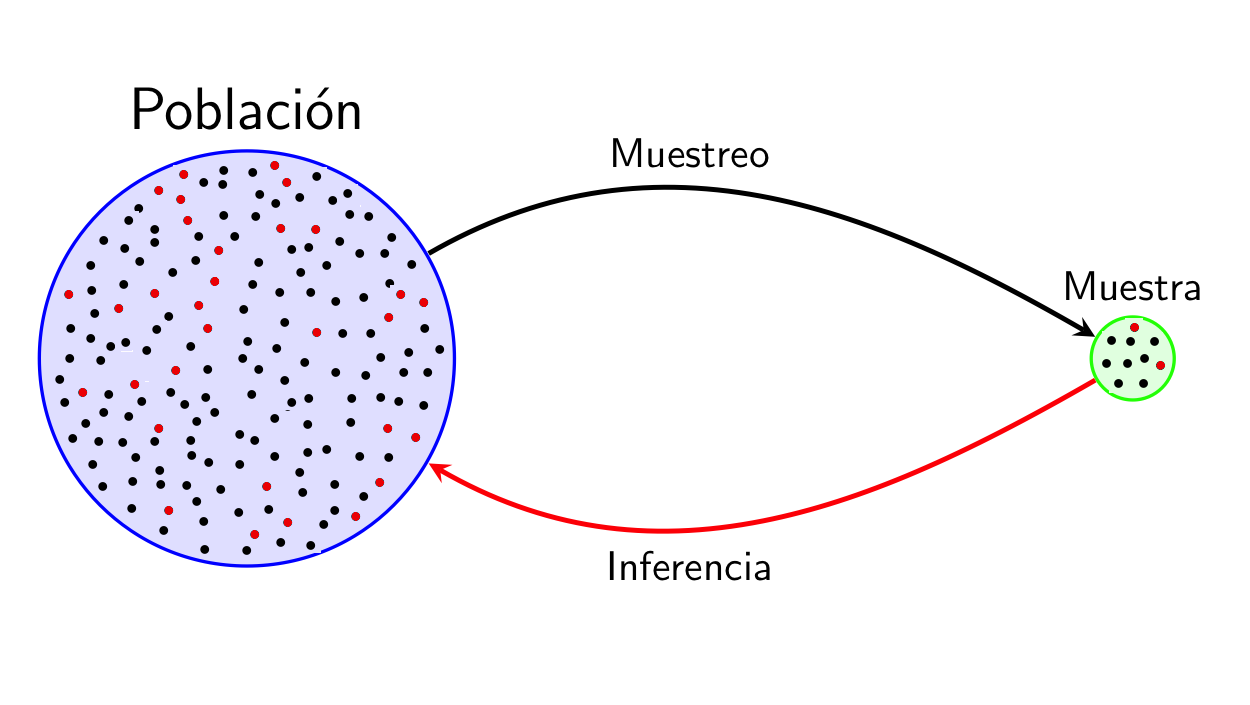
\includegraphics[width=0.8\textwidth,height=\textheight]{Figuras/EstInf.png}

}

\end{figure}

Ambos tipos de análisis están relacionados. Por un lado, porque es
conveniente (obligatorio, en nuestra opinión) empezar cualquier análisis
inferencial dando un vistazo a los datos que se usarán.

Por otro, porque muchas técnicas descriptivas permiten estimar
propiedades de la población de la que se ha extraído la muestra. Por
citar un ejemplo, la media aritmética de las alturas de un grupo de
individuos nos da un valor más o menos representativo de sus alturas,
pero también sirve para \emph{estimar} la altura media de los individuos
de la población total.

La estadística inferencial entra en juego cuando se quiere obtener
información sobre una población y no se puede acceder a todos sus
integrantes. Si por ejemplo queremos conocer la altura media de los
estudiantes matriculados en esta asignatura de la UIB en este curso, en
principio no necesitamos para nada la estadística inferencial. Sois
pocos, os mediríamos a todos y calcularíamos la media. En todo caso,
usaríamos técnicas de estadística descriptiva para arropar este valor
representando la distribución de vuestras alturas de manera adecuada.

Pero si quisiéramos conocer la altura media de los mallorquines entre 18
y 25 años, sería muy complicado medirlos a todos. Entonces, lo que
haríamos sería tomar una muestra representativa de esta población,
medirlos y a partir de sus alturas estimar dicha altura media.
Naturalmente, lo más seguro es que de esta manera no obtuviéramos el
valor exacto de la altura media de los mallorquines de 18 años, nos
tendríamos que conformar con obtener una aproximación dentro de un
cierto margen de error y determinar la probabilidad de acertar con
nuestra estimación y este margen de error. La estadística inferencial es
la que nos permite acotar el error que podamos haber cometido y calcular
la probabilidad de cometerlo, incluyendo la metodología que tendríamos
que haber usado para tomar la muestra en primer lugar.

\hypertarget{r-rstudio---posit-rmarkdowm---quarto}{%
\subsection{2.2. R/ RStudio - Posit / RMarkdowm -
Quarto}\label{r-rstudio---posit-rmarkdowm---quarto}}

Todas las técnicas que usaremos en la asignatura pueden ser
implementadas y/o desarrolladas en software libre como Python y R. Ambos
se consideran lenguajes de programación esenciales para la ciencia de
datos. Lo ideal sería dominar ambos para tener una base de programación
completa, pero:

\begin{itemize}
\item
  R es un \textbf{lenguaje específico utilizado para el análisis de
  datos y la estadística}.
\item
  R es muy adecuado para un sub-campo del aprendizaje automático
  conocido como aprendizaje estadístico. Cualquier persona con una
  formación formal en estadística debería reconocer la sintaxis y la
  construcción de R.
\item
  Al igual que Python, R cuenta con una sólida comunidad, estructurada
  alrededor de la ``Comprehensive R Archive Network'', o CRAN, pero no
  ofrece un desarrollo de software de propósito general como Python.
\item
  Cada día salen nuevos paquetes que extienden las funcionalidades de R
  y cubren casi todas las necesidades computacionales y estadísticas de
  un científico. Para que os hagáis una idea, en el momento de revisar
  estas notas (septiembre de 2023) el número de paquetes en el
  repositorio de la CRAN acaba de superar los 19800.
\item
  El acceso a R se proporciona a través de RStudio, entorno que presenta
  una ventana de visualización, un explorador de archivos, un visor de
  datos y un editor. Este entorno suele ser menos intimidante que el
  shell de R. Además, cuenta con ayuda integrada, resaltado de sintaxis
  y completado contextual por tabulaciones; todas estas herramientas
  facilitan el trabajo.
\item
  RStudio tiene un nuevo nombre desde julio de 2022: \textbf{Posit}.
  Posit es una palabra que significa proponer una idea para su
  discusión, proviene de la aspiración científica de construir niveles
  cada vez mayores de conocimiento y comprensión de experimentos que
  generan
\end{itemize}

\begin{figure}

{\centering 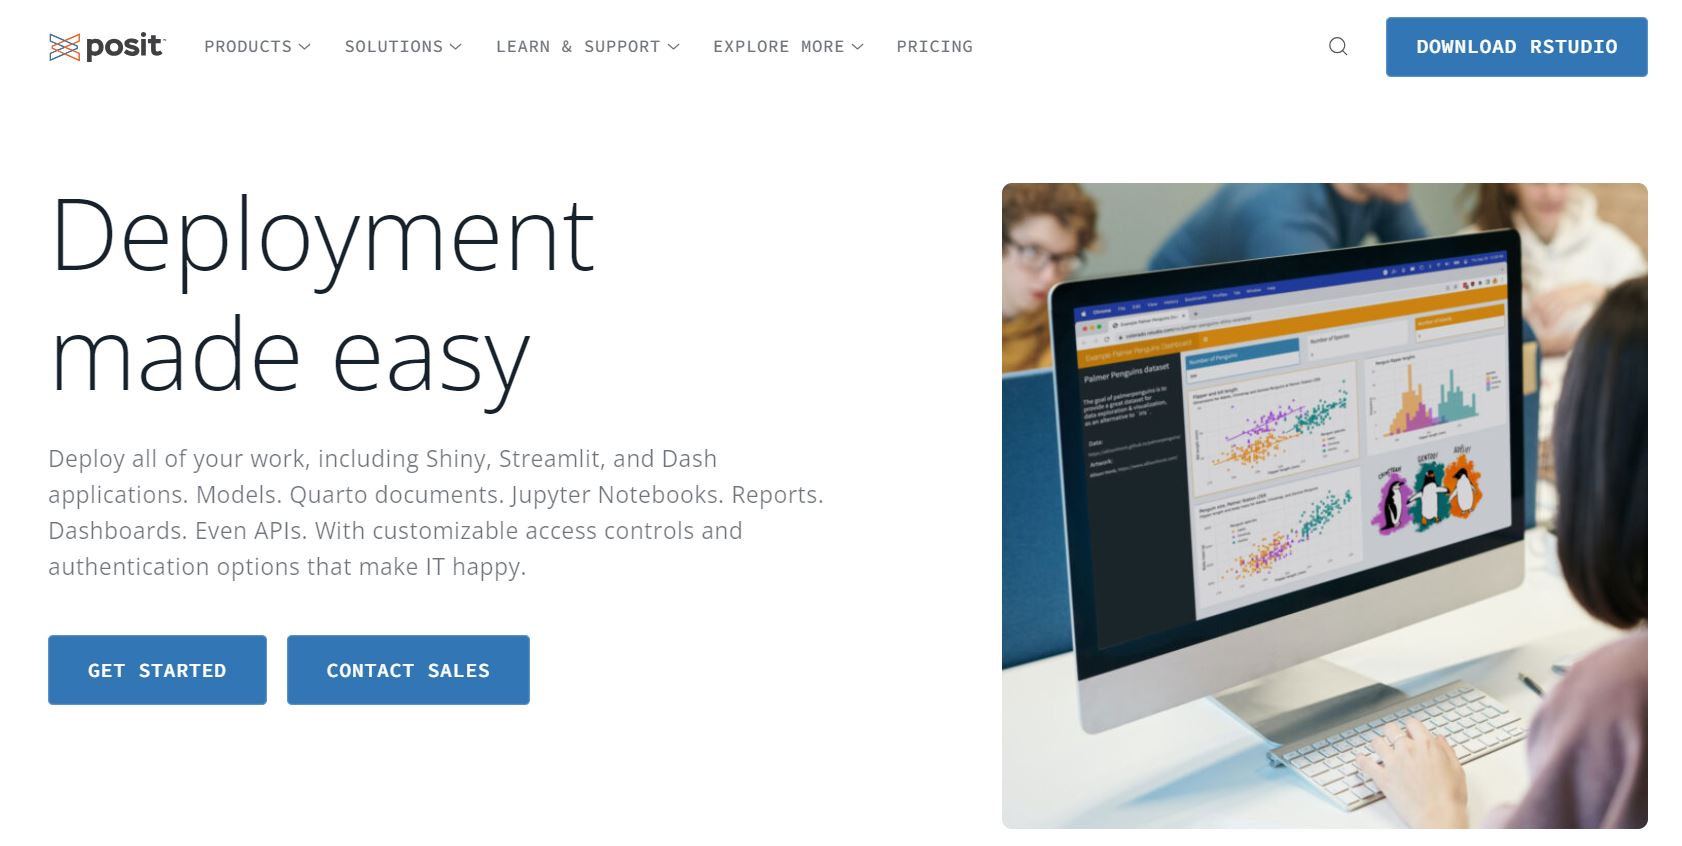
\includegraphics[width=0.8\textwidth,height=\textheight]{Figuras/posit.JPG}

}

\end{figure}

\begin{itemize}
\item
  Posit tiene como misión la creación de software libre y de código
  abierto para la ciencia de datos, la investigación científica y la
  comunicación técnica. Han incluido algunas herramientas para Python a
  través de \textbf{Quarto}.
\item
  Quarto está pensado como un cuaderno de laboratorio moderno donde
  predomina R pero que soporta código Python (\texttt{reticulate}), SQL,
  Julia, entre otros; pensado para experimentos que requieren
  multilenguaje.
\item
  \textbf{Posit Cloud} permite acceder al potente conjunto de
  herramientas de ciencia de datos de Posit directamente desde su
  navegador. Esto favorecerá el trabajo en equipo. Podéis revisar la
  siguiente \href{https://posit.cloud/learn/guide}{Guía} para crearos
  una cuenta.
\end{itemize}

\hypertarget{control-de-versiones-con-git-github}{%
\subsection{2.3. Control de versiones con Git /
GitHub}\label{control-de-versiones-con-git-github}}

\begin{itemize}
\item
  En esta asignatura la forma de llegar a un resultado de análisis de
  datos es tan importante como el propio resultado. Además, uno de los
  objetivos es exponeros al uso de herramientas de software para la
  ciencia de datos moderna.
\item
  La idea de reproducibilidad lleva implícita la colaboración. El código
  que se produce es parte de la documentación del proceso y es
  fundamental compartirlo (aunque sólo sea con uno mismo).
\item
  Lo anterior se logra mejor con un sistema de control de versiones
  distribuido como \textbf{Git}. Mantener un registro sobre los
  proyectos, es lo que permite rastrear y gestionar cambios en el código
  a lo largo del tiempo. Se puede decir que nos permite guardar el
  progreso de nuestro código de tal forma que, si en algún momento
  cometemos algún error irreversible en una versión posterior, siempre
  podremos recuperar una versión anterior en la que todo funcionaba
  correctamente y retomar el proyecto desde ese punto.
\item
  Git permite la colaboración, pero carece de características sociales y
  herramientas específicas para la colaboración en equipo.
  \textbf{GitHub} proporciona herramientas para la revisión de código,
  la gestión de problemas y la colaboración en proyectos.
\end{itemize}

\begin{figure}

{\centering 
\includegraphics[width=0.5\textwidth,height=\textheight]{Figuras/GitHub.png}

}

\end{figure}

\begin{itemize}
\item
  GitHub es un servicio en la nube donde se pueden subir repositorios
  propios y compartir el código con otras personas de tal forma que sea
  accesible desde Internet.
\item
  Un repositorio funciona como una carpeta virtual. En él se encuentran
  todos los archivos de un proyecto y el historial de revisiones de cada
  uno, permitiendo restablecer una versión del código en caso de error
  en su ejecución.
\item
  Podemos ver proyectos de otras usuarios, valorarlos, proponer mejoras
  en el código, GitHub es una de las aplicaciones que mejora la gestión
  de proyectos y el acceso a recursos compartidos.
\item
  En octubre del 2021 se estrenó \textbf{GitHub Copilot}, una
  herramienta de inteligencia artificial en la nube desarrollada
  conjuntamente entre GitHub y OpenAI. Su objetivo es sugerir y
  autocompletar el código escrito en entornos de desarrollo integrados
  (IDE).
\end{itemize}

\begin{quote}
En esta clase, utilizaremos GitHub como sistema de gestión del
aprendizaje para distribuir y recopilar las entregas como repositorios.
\end{quote}

\begin{itemize}
\tightlist
\item
  Crearemos en GitHub un repositorio por estudiante/equipo para cada
  entrega. Utilizaremos un sencillo flujo de trabajo centralizado que
  sólo requiere realizar acciones simples como push, pull, add, rm,
  commit, status y clone.
\end{itemize}

\hypertarget{git-github-con-r}{%
\subsection{2.4. Git / GitHub con R}\label{git-github-con-r}}

Veamos cómo configurar todo. Gran parte de lo que está aquí proviene del
libro \href{https://happygitwithr.com/}{Happy Git and GitHub for the
useR} de Jenny Bryan y del artículo de
\href{https://rfortherestofus.com/2021/02/how-to-use-git-github-with-r/}{David
Keyes} puedes ver sus vídeos en caso de que, la breve explicación que
presentamos abajo, no sea suficiente para ti.

\begin{itemize}
\tightlist
\item
  {\emph{Instalar Git}}: El primer paso es instalar Git, en el
  \href{https://happygitwithr.com/install-git}{Capítulo 6 del libro}
  explican el proceso para los usuarios de Mac, Windows y Linux.
  Nosotros ya lo tenemos instalado, así que mostramos cómo verificar si
  tienes Git instalado y su versión usando el terminal en RStudio.
\end{itemize}

En el terminal de RStudio:

\begin{Shaded}
\begin{Highlighting}[]
\NormalTok{which git }\CommentTok{\# ruta donde está instalado el Git}
\NormalTok{git }\SpecialCharTok{{-}{-}}\NormalTok{version }\CommentTok{\# version}
\end{Highlighting}
\end{Shaded}

\begin{itemize}
\tightlist
\item
  {\emph{Configurar Git (Editar gitconfig file)}}:El siguiente paso es
  configurar Git. Esto se trata en el Capítulo 7 del libro, aunque
  mostramos lo que creemos es un proceso un poco más fácil.
  Específicamente, sugerimos usar la función
  \texttt{edit\_git\_config()} del paquete \texttt{usethis}, que abrirá
  su archivo gitconfig. Agrega tu nombre y correo electrónico y cierra
  esto.
\end{itemize}

En la consola de RStudio:

\begin{Shaded}
\begin{Highlighting}[]
\FunctionTok{library}\NormalTok{(usethis)}
\NormalTok{usethis}\SpecialCharTok{::}\FunctionTok{edit\_git\_config}\NormalTok{()}
\CommentTok{\# Modificar en el fichero ".gitconfig" los apartados: "name" y "email" }
\CommentTok{\# y guardar el fichero}
\end{Highlighting}
\end{Shaded}

\begin{itemize}
\tightlist
\item
  {\emph{Inicializar un repositorio Git}}: Ahora que has instalado y
  configurado Git, puedes usarlo localmente. La función
  \texttt{use\_git()} agregará un repositorio Git (a menudo denominado
  ``repositorio'') a un proyecto RStudio existente. Aquí crearemos un
  nuevo proyecto y luego inicializaremos un repositorio de Git.
\end{itemize}

En RStudio: * Crear un proyecto nuevo

\begin{itemize}
\item
  Seleccionar ``Nuevo Directorio''
\item
  Proyecto

  \begin{itemize}
  \tightlist
  \item
    Activar: ``Create a git repository''
  \end{itemize}
\end{itemize}

En la consola de RStudio:

\begin{Shaded}
\begin{Highlighting}[]
\FunctionTok{library}\NormalTok{(usethis)}
\NormalTok{usethis}\SpecialCharTok{::}\FunctionTok{use\_git}\NormalTok{()}
\CommentTok{\# Elegir siempre la opción: 1}
\CommentTok{\# Y ante la ventana, seleccionar: "Save"}
\end{Highlighting}
\end{Shaded}

Y visitar la pestaña: ``Git'' en RStudio.

\begin{itemize}
\tightlist
\item
  {\emph{Ver historial de confirmación}}: Ahora que tu proyecto de
  RStudio tiene un repositorio Git asociado, verás una pestaña adicional
  en la parte superior derecha: la pestaña Git. Desde aquí, puedes ver
  todo el historial de cambios en tu código a lo largo del tiempo
  (¡todavía no muchos!).
\end{itemize}

En RStudio:

Visitar la pestaña: ``Git'' de RStudio Pulsar el icono del reloj para
ver el historial de ``Commit'' realizados para ver el ``Initial
Commit''.

\begin{itemize}
\tightlist
\item
  {\emph{Hacer una confirmación (commit) y ver más historia}}: Git no
  realiza un seguimiento automático de los cambios de la manera en que
  lo hace una herramienta como Google Docs. En su lugar, tienes que
  decirle a Git: Hice cambios y quiero que mantengas un registro de
  ellos. Decirle a Git esto se llama hacer una confirmación (commit) y
  puedes hacerlo desde RStudio.
\end{itemize}

Cada commit tiene un mensaje de confirmación, lo que es útil porque,
cuando miras tu historial de código, ves lo que hiciste en cada momento
(es decir, en cada commit). RStudio tiene una herramienta integrada para
ver su historial de código. Puedes hacer clic en cualquier commit para
ver qué cambió, en relación con el commit anterior. Las líneas que se
agregaron en verde; y las que se eliminaron en rojo.

En RStudio:

\begin{itemize}
\item
  Crear un fichero de script R: ``test.R'' y guardarlo.
\item
  Visita la pestaña ``Git'' de RStudio y pulsa sobre el botón de
  ``commit'' para confirmar la creación del fichero: ``test.R''.
\item
  En el panel del commit añada un texto que lo defina.
\item
  Haz varios cambios en el fichero ``test.R'' y en cada uno de ellos haz
  de nuevo un ``commit''.
\item
  Revisa luego la historia de los cambios que se han producido en el
  historial (pulsar el icono del reloj).
\item
  Observa los nuevos cambios resaltados en color verde. Frente a los
  valores antiguos que aparecerán en color rojo.
\end{itemize}

\hypertarget{conectar-rstudio-y-github}{%
\subsection{2.5. Conectar RStudio y
GitHub}\label{conectar-rstudio-y-github}}

El proceso hasta ahora nos ha permitido usar Git localmente. Pero, ¿qué
pasa si queremos conectarnos a GitHub? ¿Cómo lo hacemos?

La mejor manera de conectar RStudio y GitHub es usando tu nombre de
usuario y un token de acceso personal (PAT). Para generar un token de
acceso personal, usa la función \texttt{create\_github\_token()} de
\texttt{usethis}. Esto te llevará a la página correspondiente en el
sitio web de GitHub, donde le darás un nombre a tu token y lo copiarás
(¡no lo pierdas porque nunca volverá a aparecer!).

En la consola de RStudio:

\begin{Shaded}
\begin{Highlighting}[]
\FunctionTok{library}\NormalTok{(usethis)}
\NormalTok{usethis}\SpecialCharTok{::}\FunctionTok{create\_github\_token}\NormalTok{()}
\end{Highlighting}
\end{Shaded}

\begin{itemize}
\item
  Pulsa sobre el enlace que aparece en la salida en la consola.
\item
  Se abrirá una página web de Github en la que tendrás que pulsar el
  botón ``Generate token''.
\item
  Copia el token que aparece en Github (lo utilizarás en el siguiente
  paso).
\item
  Ahora que has creado un token de acceso personal, debes almacenarlo
  para que RStudio pueda acceder a él y sepa conectarse a tu cuenta de
  GitHub. La función \texttt{gitcreds\_set()} del paquete
  \texttt{gitcreds} te ayudará aquí. Ingresará tu nombre de usuario de
  GitHub y el token de acceso personal como contraseña (NO tu contraseña
  de GitHub). Una vez que hayas hecho todo esto, ¡habrás conectado
  RStudio a GitHub!.
\end{itemize}

En la consola de RStudio:

\begin{Shaded}
\begin{Highlighting}[]
\FunctionTok{library}\NormalTok{(gitcreds)}
\NormalTok{gitcreds}\SpecialCharTok{::}\FunctionTok{gitcreds\_set}\NormalTok{()}
\CommentTok{\# Ante la pregunta: "Enter password or token"}
\CommentTok{\# introduce el token copiado en el paso anterior}
\end{Highlighting}
\end{Shaded}

\hypertarget{conectar-proyectos-de-rstudio-con-repositorios-de-github}{%
\subsection{2.6. Conectar proyectos de RStudio con repositorios de
GitHub}\label{conectar-proyectos-de-rstudio-con-repositorios-de-github}}

Ahora que hemos conectado RStudio y GitHub, discutamos cómo hacer que
los dos funcionen juntos. La idea básica es que configures los proyectos
que creas en RStudio con repositorios GitHub asociados. Cada proyecto de
RStudio vive en un solo repositorio de GitHub.

¿Cómo conectamos un proyecto de RStudio a un repositorio de GitHub?
Happy Git and GitHub for the useR propone tres estrategias.
Demostraremos la forma más sencilla

crear un repositorio en GitHub primero. Cree el repositorio y, a
continuación, cuando inicie un nuevo proyecto en RStudio, utilice la
opción de control de versiones, introduzca la URL de su repositorio y
listo.

\textbf{GitHub primero}

Crea el repositorio en GitHub y, a continuación, cuando inicies un nuevo
proyecto en RStudio, utiliza la opción de control de versiones,
introduce la URL de tu repositorio y listo.

Para bajar un repositorio creado en Github a un proyecto local en
RStudio, tendréis que realizar los siguientes pasos:

\begin{itemize}
\item
  Crear un nuevo repositorio en nuestra cuenta de Github (o utilizar uno
  ya existente): pulsar el botón ``Create repository''.
\item
  Copiar al portapapeles la primera dirección que aparece (pulsando el
  botón de la derecha). Coincide con la dirección url que aparece en la
  barra del navegador.
\item
  En RStudio seleccionamos crear ``New project'', elegimos ``Version
  Control'' y luego seleccionamos ``Git''.
\item
  Introducimos en el primer cuadro de texto la url copiada
  anteriormente. Pulsamos ``Create Project''.
\item
  A continuación podrás consultarse la pestaña ``Git'' y ver la
  información asociada al repositorio descargado.
\end{itemize}

\hypertarget{flujo-de-trabajo-general}{%
\subsection{2.7. Flujo de trabajo
general}\label{flujo-de-trabajo-general}}

Ahora que hemos conectado RStudio y GitHub, podemos compartir nuestro
trabajo entre los dos.

\textbf{Push (Subir a Github)}

``Push'' significa enviar cualquier cambio en tu código de RStudio a
GitHub. Para hacer esto, primero tenemos que hacer un commit. Después de
confirmar, ahora tenemos un botón (la flecha hacia arriba) en RStudio
que podemos usar para enviar nuestro código a GitHub.

En RStudio:

\begin{itemize}
\item
  Creamos un nuevo fichero de script R o un fichero Rmd y lo guardamos.
\item
  Pulsamos en la pestaña ``Git'' sobre el botón de ``commit''. Marcamos
  todos los ficheros sobre los checks de ``Staged'', rellenamos la
  descripción del commit y pulsamos sobre el botón de ``commit''.
\item
  Después de hacer el commit, pulsamos sobre el botón ``Push'' para
  subir los cambios a Github.
\item
  A continuación puedes comprobar en la página de Github del repositorio
  que se han actualizado los últimos ficheros considerados en el último
  commit.
\end{itemize}

\textbf{Pull (Descargar desde Github)}

Lo opuesto a ``empujar''Push'' es bajar (``Pull''). Utilizando el botón
de flecha hacia abajo, RStudio va al repositorio de GitHub, toma el
código más reciente y lo lleva a su editor local.

Hacer ``Push'' regularmente es extremadamente importante si estás
colaborando, aunque si eres el único que trabaja en un proyecto de
RStudio y un repositorio GitHub asociado, sabes que tu código local
coincide con lo que está en GitHub, por lo que es menos importante.

En la página de Github de nuestro repositorio:

\begin{itemize}
\item
  Editamos uno de los ficheros de nuestro repositorio pulsando sobre el
  icono de un lápiz (a la derecha). Realizamos alguna modificación sobre
  el fichero (o ficheros).
\item
  Pulsamos en la parte inferior de la página en el botón de ``Commit
  changes'' (rellenando los comentarios que creamos oportunos sobre el
  commit que se está realizando). Se puede navegar por la página de
  Github para consultar todos los commits realizados (y mucha más
  información).
\end{itemize}

Volvemos a RStudio:

\begin{itemize}
\item
  En la pestaña ``Git'' pulsamos sobre el botón de la flecha que apunta
  hacia abajo (verde) para realizar un ``Pull'' o descarga de los
  cambios en Github a nuestro proyecto local en RStudio.
\item
  Después de eso puedes comprobare que los ficheros locales de nuestro
  proyecto se han actualizado con los cambios que se han producido en el
  repositorio.
\end{itemize}

\textbf{¡Lo lograste!}

¡Ahora está todo configurado para usar Git y GitHub con RStudio!

\hypertarget{los-datos-y-sus-tipos}{%
\section{3. Los datos y sus tipos}\label{los-datos-y-sus-tipos}}

En vuestro curso de Estadística estudiasteis algunas técnicas básicas de
estadística descriptiva. Estas técnicas consisten en una serie de
valores y gráficos que nos permiten resumir y explorar un conjunto de
datos, con el objetivo final de entenderlos o describirlos lo mejor
posible.

Los datos de los que disponemos suelen ser multidimensionales, en el
sentido de que observamos varias características (\textbf{variables}) de
una serie de individuos. Almacenamos estos datos en \textbf{tablas de
datos} como la que presentamos abajo, donde cada columna corresponde a
una variable y cada fila son los datos de un individuo concreto. Así, en
esta tabla, cada fila representa un niño y cada columna recoge una de
las características que hemos anotado: su nombre, su altura (en cm), su
número de hermanos, el color de sus cabellos, el número semanal de
refrescos que suele tomar, y su grado de satisfacción con un juego para
móvil (entre 0 y 5).

\begin{table}

\caption{Una pequeña tabla de datos sobre niños}
\centering
\begin{tabular}[t]{l|l|r|r|l|l|r}
\hline
  & Nombre & Altura & Hermanos & Cabello & Refrescos semanales & Satisfacción App\\
\hline
1 & Marta & 135 & 2 & rubio & 2-3 & 4\\
\hline
2 & Laura & 132 & 1 & negro & 2-3 & 4\\
\hline
3 & Xavier & 138 & 0 & negro & 0-1 & 3\\
\hline
4 & Joan & 141 & 3 & castaño & 4-5 & 2\\
\hline
5 & Maria & 134 & 2 & rojo & 0-1 & 3\\
\hline
6 & Maria & 136 & 1 & castaño & 6 o más & 5\\
\hline
\end{tabular}
\end{table}

\BeginKnitrBlock{rmdcaution}

En este curso vamos a ``sobrecargar'' el término \textbf{variable}, en
el sentido de que tendrá dos significados diferentes que esperamos que
podáis distinguir según el contexto:

\begin{itemize}
\item
  Por un lado, llamaremos \textbf{variable} a una característica que
  puede tomar diferentes valores sobre diferentes individuos; cuando
  tenga este sentido, a veces le añadiremos el adjetivo
  \textbf{poblacional}. Por ejemplo, la altura de las personas (de todo
  el mundo, de un país, de una ciudad\ldots) es una variable
  poblacional.
\item
  Por otro lado, también llamaremos una \textbf{variable} a un vector
  formado por los valores de una variable poblacional sobre los sujetos
  de una muestra. Por ejemplo, las alturas de los niños recogidas en la
  tabla forman una variable en este sentido.
\end{itemize}

\EndKnitrBlock{rmdcaution}

Los tipos básicos de datos que consideramos en este curso son los
siguientes:

\begin{itemize}
\item
  Datos \textbf{cualitativos}. Son los que expresan una cualidad del
  individuo, como por ejemplo el sexo cromosómico (macho, hembra), el
  género de una persona (hombre, mujer, lesbiana, gay, bisexual,
  transexual, intersexual, asexual), tipos de cáncer (de mama, de colon,
  de próstata\ldots)\ldots{} Si solo pueden tomar dos valores (``Sí'' o
  ``No'', ``Macho'' o ``Hembra''\ldots) los llamamos \textbf{binarios} o
  \textbf{dicotómicos} y si pueden tomar más de dos valores,
  \textbf{politómicos} o \textbf{multicotómicos}, dependiendo de lo que
  queramos complicar los adjetivos. A los posibles valores que puede
  tomar un tipo de datos cualitativo se los suele llamar
  \textbf{niveles}.

  Los datos cualitativos pueden ser iguales o distintos, y no admiten
  ningún otro tipo de comparación.
\item
  Datos \textbf{ordinales}. Son datos similares a los cualitativos, en
  el sentido de que expresan una cualidad del individuo, pero con la
  diferencia de que se pueden ordenar de manera natural. Por ejemplo,
  los niveles de gravedad de una enfermedad (sano, leve, grave, muy
  grave, \ldots) o las calificaciones en un examen (suspenso, aprobado,
  notable, sobresaliente) son datos ordinales. En cambio, no se pueden
  ordenar de manera significativa los sexos o los tipos de cáncer de los
  individuos: por eso son datos cualitativos y no ordinales.

  También se suele llamar a los posibles valores que puede tomar un tipo
  de datos ordinal sus \textbf{niveles}.
\item
  Datos \textbf{cuantitativos}. Son datos que se refieren a medidas que
  sean números genuinos, con los que tenga sentido operar, tales como
  edades, longitudes, pesos, tiempos, números de individuos, etc.
  Distinguimos dos tipos:

  \begin{itemize}
  \item
    \textbf{Discretos}: Pueden tomar solo valores que avanzan a saltos y
    que podemos identificar con números naturales: número de hermanos,
    número de ingresos en un día en un hospital\ldots{}
  \item
    \textbf{Continuos}: Podrían tomar cualquier valor real dentro de un
    intervalo si se pudieran medir con precisión infinita: altura,
    temperatura, tiempo\ldots{}
  \end{itemize}
\end{itemize}

\begin{Shaded}
\begin{Highlighting}[]
\NormalTok{En la tabla anterior:}
  
\NormalTok{* La variable "Nombre" es cualitativa.}
\NormalTok{* La variable "Altura" es cuantitativa continua.}
\NormalTok{* La variable "Hermanos" es cuantitativa discreta.}
\NormalTok{* La variable "Cabello" es cualitativa.}
\NormalTok{* La variable "Refrescos semanales" es ordinal.}
\NormalTok{* La variable "Satisfacción App" también es ordinal.}
\end{Highlighting}
\end{Shaded}

Dos puntos relevantes a tener en cuenta y que justifican algunas
clasificaciones que puede que encontréis dudosas en el ejemplo anterior:

\begin{itemize}
\item
  \textbf{No todo número es un dato cuantitativo.} Solo los consideramos
  cuantitativos cuando son números genuinos, ``de verdad''. Por ejemplo,
  si pedimos a un paciente que califique su dolor con un número natural
  de 0 a 10, no es un dato cuantitativo, sino ordinal:

  \begin{itemize}
  \item
    No es una medida precisa del dolor; no son números ``de verdad'',
    sino abreviaturas de ``Nada'', ``Un poquito'',\ldots, ``Matadme''.
  \item
    Tener dolor 6 no significa ``tener el doble de dolor'' que tener
    dolor 3 (si lo significara, ¿cuál sería el valor correspondiente
    ``al doble de dolor'' que 7?). En cambio, una persona con 6 hermanos
    sí que tiene el doble de hermanos que si tuviera 3.
  \item
    No tiene sentido sumarlos u operarlos en general. Por ejemplo, si yo
    tengo dolor de nivel 6 y tú tienes dolor de nivel 5, entre los dos
    no tenemos dolor de nivel 11. En cambio, si yo tengo 6 hermanos y tú
    5, entre los dos sí que tenemos 11 hermanos.
  \end{itemize}

  Este es justamente el caso de la variable ``Satisfacción App'' de la
  tabla anterior. Pese a que sus valores son números, el único contenido
  real que tienen es su orden: a la María que toma muchos refrescos le
  ha gustado la app bastante más que a la María que apenas toma
  refrescos.
\item
  \textbf{La distinción discreto-continuo es puramente teórica}. En
  realidad, todo dato es discreto porque no podemos medir nada con
  precisión infinita, pero las herramientas matemáticas ``continuas''
  (derivadas, integrales, etc.) son mucho más potentes que las
  discretas, por lo que siempre que tenga sentido, es conveniente
  considerar una variable como continua.

  Observad, por ejemplo, la diferencia entre la altura, pongamos que
  medida en cm y redondeada a unidades como en la tabla anterior, y el
  número de hermanos. Ambos se presentan como números naturales, pero
  los números de hermanos no admiten mayor precisión, mientras que las
  alturas las podríamos medir, con los aparatos adecuados, en mm, en µm,
  en nm\ldots. Como además las herramientas para tratar datos continuos
  son mucho más potentes, vamos a considerar las alturas como datos
  continuos, mientras que los números de hermanos no hay más remedio que
  tratarlos como discretos.

  En concreto, \textbf{es conveniente considerar en la práctica como
  datos continuos aquellos que dan lugar a números naturales muy
  grandes}, como por ejemplo los números de glóbulos rojos en un litro
  de sangre, de bases nucléicas en un genoma, o de personas de un país.
  La diferencia entre diez millones, diez millones uno, diez millones
  dos\ldots{} puede considerarse como continua: de hecho, si tomamos el
  millón como unidad, la diferencia está en la séptima cifra decimal.
\end{itemize}

\BeginKnitrBlock{rmdnote}

Hemos dicho que la variable ``Cabello'' es cualitativa. En principio, el
color de los cabellos no tiene ningún orden ``natural''. Pero si en un
estudio definimos un orden claro para esta variable (por ejemplo, por la
longitud de onda correspondiente) y este orden es relevante en nuestro
estudio, habrá que considerarla una variable ordinal.
\EndKnitrBlock{rmdnote}

\BeginKnitrBlock{rmdnote}

La variable ``Refrescos semanales'' es de un tipo de datos ordinales muy
concreto que a veces se califican de \textbf{cuantitativos agrupados}:
sus niveles se obtienen agrupando en intervalos los posibles valores de
una variable cuantitativa (en este caso, la variable discreta que mide
el número preciso de refrescos semanales). \EndKnitrBlock{rmdnote}

\begin{quote}
El análisis, tanto descriptivo como inferencial, de un conjunto de datos
es diferente según su tipo.
\end{quote}

Así, para datos cualitativos sólo tiene interés estudiar y representar
las frecuencias con que aparecen sus diferentes valores, mientras que el
análisis de datos cuantitativos suele involucrar el cálculo de medidas
estadísticas, como la media o la desviación típica, que expresen
numéricamente sus propiedades.

Os dejamos el material
\href{https://aprender-uib.github.io/AprendeR1/}{Aprender R1} para que
repaséis los capítulos 10 al 14 correspondientes a la parte de
Estadística descriptiva.

\hypertarget{pruxe1ctica-1}{%
\section{\texorpdfstring{4. {\emph{Práctica
1}}:}{4. Práctica 1:}}\label{pruxe1ctica-1}}

\begin{itemize}
\item
  Formad grupos de 3 integrantes.
\item
  Trabajaréis con los datos
  \href{https://allisonhorst.github.io/palmerpenguins/}{pingüinos}, leed
  la documentación y seguid las siguientes instrucciones:

  \begin{itemize}
  \item
    Cread un repositorio en Github para vuestro grupo con un nombre que
    sea fácilmente identificable para los profesores de la asignatura,
    por ejemplo,``Entrega\_1\_AD''.
  \item
    Cread un proyecto nuevo en RStudio conectado al repositorio que
    habéis creado en el paso anterior. Agregad un documento de quarto
    donde trabajaréis.
  \item
    Instalad y cargad en RStudio la librería \texttt{palmerpenguins} ,
    así como el conjunto de datos \texttt{penguins}
  \end{itemize}
\end{itemize}

\begin{Shaded}
\begin{Highlighting}[]
\CommentTok{\#install.packages("palmerpenguins",dep=TRUE)}
\FunctionTok{library}\NormalTok{(}\StringTok{"palmerpenguins"}\NormalTok{)}
\FunctionTok{print}\NormalTok{(penguins, }\AttributeTok{width =} \DecValTok{50}\NormalTok{)}
\end{Highlighting}
\end{Shaded}

\begin{verbatim}
# A tibble: 344 x 8
   species island    bill_length_mm bill_depth_mm
   <fct>   <fct>              <dbl>         <dbl>
 1 Adelie  Torgersen           39.1          18.7
 2 Adelie  Torgersen           39.5          17.4
 3 Adelie  Torgersen           40.3          18  
 4 Adelie  Torgersen           NA            NA  
 5 Adelie  Torgersen           36.7          19.3
 6 Adelie  Torgersen           39.3          20.6
 7 Adelie  Torgersen           38.9          17.8
 8 Adelie  Torgersen           39.2          19.6
 9 Adelie  Torgersen           34.1          18.1
10 Adelie  Torgersen           42            20.2
# i 334 more rows
# i 4 more variables: flipper_length_mm <int>,
#   body_mass_g <int>, sex <fct>, year <int>
\end{verbatim}

\begin{figure}

{\centering 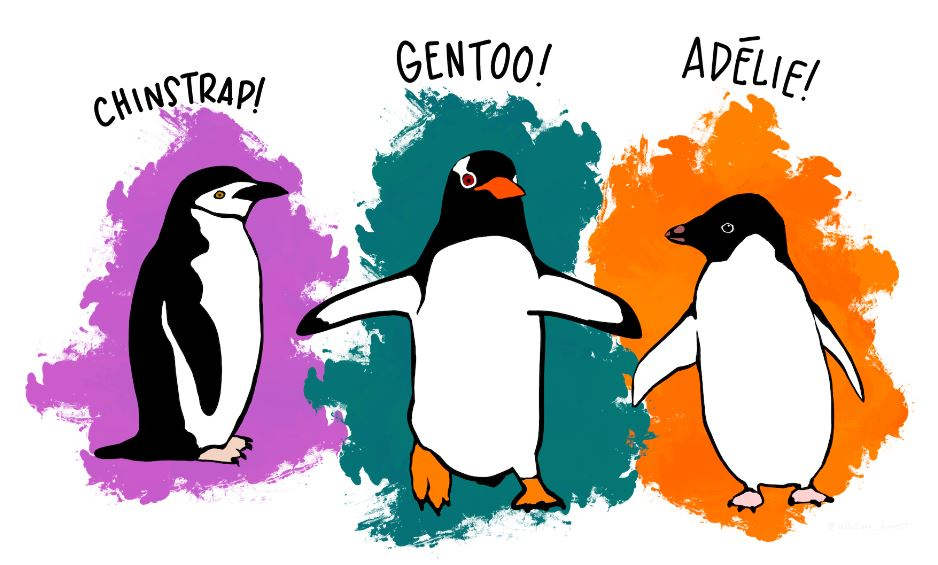
\includegraphics[width=0.6\textwidth,height=\textheight]{Figuras/pinguinos_madagascar.jpg}

}

\end{figure}

\begin{itemize}
\item
  Con lo que sabéis de R base, realizad un análisis exploratorio de
  datos y redactad un reporte con los hallazgos más importantes. No
  olvidéis agregar en el reporte el URL de vuestro repositorio de
  GitHub.
\item
  Entregad el reporte en la tarea de Aula Digital disponible. Revisad la
  fecha en que cierra la tarea.
\end{itemize}

\hypertarget{gramuxe1tica-limpia-y-coherente-con-tidyverse}{%
\section{\texorpdfstring{5. Gramática limpia y coherente con
\texttt{Tidyverse}}{5. Gramática limpia y coherente con Tidyverse}}\label{gramuxe1tica-limpia-y-coherente-con-tidyverse}}

\hypertarget{la-libreruxeda-tidyverse}{%
\subsection{\texorpdfstring{5.1. La librería
\texttt{Tidyverse}}{5.1. La librería Tidyverse}}\label{la-libreruxeda-tidyverse}}

\begin{figure}

{\centering 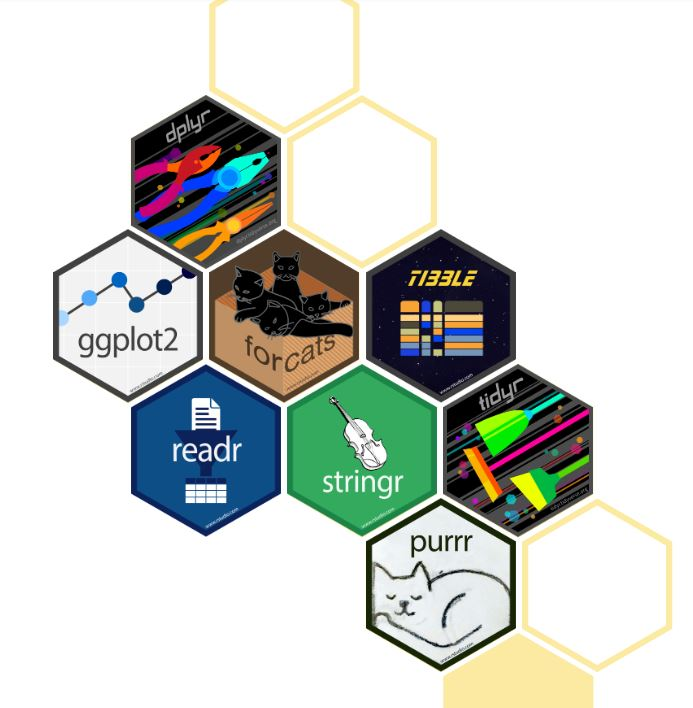
\includegraphics[width=0.4\textwidth,height=\textheight]{Figuras/tidyverse-hex.PNG}

}

\end{figure}

\begin{itemize}
\item
  \textbf{Tidyverse} es una colección de paquetes/librerías de R para
  ciencia de datos que comparten una filosofía de diseño, gramática y
  estructuras similar. En la página
  \href{https://www.tidyverse.org/}{Tidverse.org} podéis encontrar una
  descripción detallada de cada una de las librerías, un Blog con
  artículos de interés para la ciencia de datos, ayuda y recursos de
  aprendizaje.
\item
  Todos estos paquetes están pensados para:

  \begin{itemize}
  \item
    Tener una tecnología con la que puedan convivir diferentes tipos de
    profesionales (como por ejemplo: informáticos, economistas,
    matemáticos, gestores) compartiendo el mismo flujo de datos.
  \item
    Facilitar el análisis y modelización de datos
  \end{itemize}
\end{itemize}

\begin{figure}

{\centering 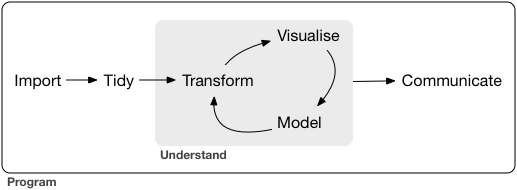
\includegraphics[width=0.6\textwidth,height=\textheight]{Figuras/data-science.png}

}

\end{figure}

\begin{itemize}
\item
  \href{https://hadley.nz/}{Hadley Wickham}, su creador, es el director
  de los científicos de datos de RStudio (actual Posit) y profesor
  adjunto de estadística en la Universidad de Auckland, la Universidad
  de Stanford y la Universidad de Rice.
\item
  Las librerías de tidyverse han venido a sustituir R base por su
  eficiencia y facilidad de programación para no informáticos. Casi
  todas las consultas a páginas técnicas de R son o incluyen código de
  \texttt{tidyverse}.
\item
  \textbf{Paquetes de \texttt{tidyverse} base :}

  \begin{itemize}
  \tightlist
  \item
    \texttt{readr}: lectura de datos
  \item
    \texttt{tibble}: una clase `tbl\_df' que constituye un mejor formato
    que el data frame tradicional.
  \item
    \texttt{stringr}: paquete de funciones para texto
  \item
    \texttt{forcats}: paquete de funciones para factores
  \item
    \texttt{tidyr}: arreglo y limpieza de datos
  \item
    \texttt{dplyr}: manipulación de datos
  \item
    \texttt{ggplot2}: visualización (gráficos)
  \item
    \texttt{purrr}: programación funcional (pipes)
  \end{itemize}

  Hay muchos otros paquetes que se integran sin problemas, por ejemplo,
  \texttt{lubridate} (para manejar datos tomados en el tiempo),
  \texttt{stringr} (texto), \texttt{forcats} (factores), etc.
\item
  Para instalar y cargar \texttt{tidyverse}
\end{itemize}

\begin{Shaded}
\begin{Highlighting}[]
\CommentTok{\#install.packages("tidyverse")}
\FunctionTok{library}\NormalTok{(tidyverse)}
\end{Highlighting}
\end{Shaded}

\begin{verbatim}
-- Attaching core tidyverse packages ------------------------ tidyverse 2.0.0 --
v dplyr     1.1.2     v readr     2.1.4
v forcats   1.0.0     v stringr   1.5.0
v ggplot2   3.4.2     v tibble    3.2.1
v lubridate 1.9.2     v tidyr     1.3.0
v purrr     1.0.1     
-- Conflicts ------------------------------------------ tidyverse_conflicts() --
x dplyr::filter()     masks stats::filter()
x dplyr::group_rows() masks kableExtra::group_rows()
x dplyr::lag()        masks stats::lag()
i Use the conflicted package (<http://conflicted.r-lib.org/>) to force all conflicts to become errors
\end{verbatim}

Se puede ver la versión del paquete tidyverse y la de los paquetes base.

{Cuidado}: algunas funciones de R se sobrescriben por sus equivalentes
de \texttt{tidyverse}. En ocasiones es preferible indicar explícitamente
el nombre de la función que deseamos utilizar, por ejemplo:
\texttt{dplyr::group\_by} para distinguir de \texttt{plyr::group\_by}
(dplyr es una evolución del paquete plyr).

\hypertarget{quuxe9-significa-tidy-data}{%
\subsection{5.2. ¿Qué significa tidy
data?}\label{quuxe9-significa-tidy-data}}

\begin{figure}

{\centering 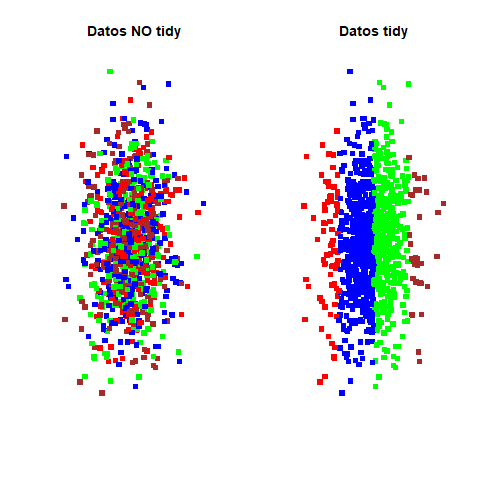
\includegraphics[width=0.5\textwidth,height=\textheight]{Figuras/plot_tidy.png}

}

\end{figure}

\begin{itemize}
\item
  Decimos que unos datos están bien estructurados o son ``tidy data'' si
  se cumplen los siguientes principios:

  \begin{itemize}
  \item
    Cada variable forma una columna.
  \item
    Cada observación forma una fila.
  \item
    Cada tipo de unidad de observación forma una tabla.
  \end{itemize}
\end{itemize}

\begin{figure}

{\centering 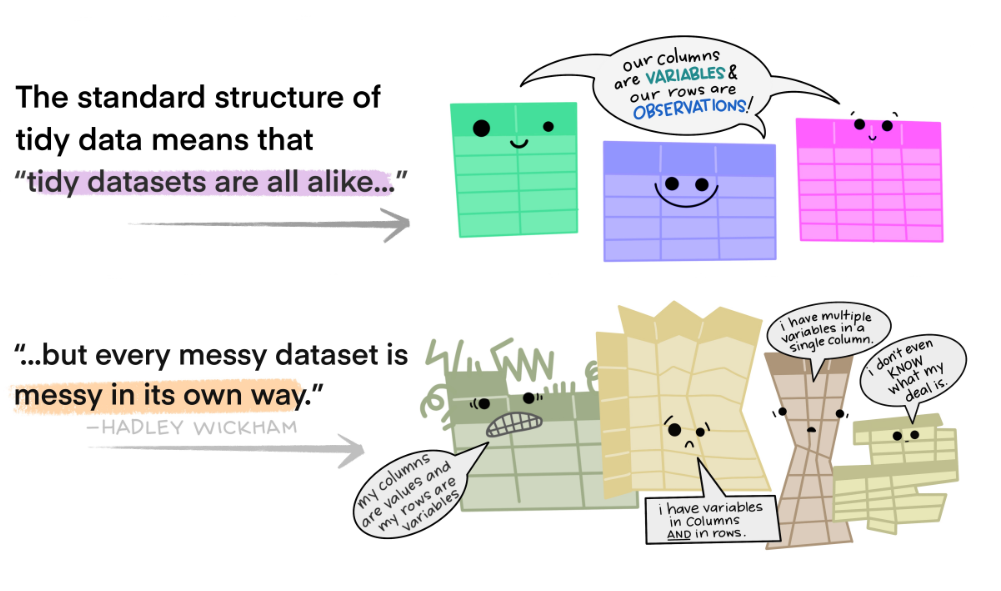
\includegraphics[width=0.6\textwidth,height=\textheight]{Figuras/tidy_data.PNG}

}

\end{figure}

\begin{itemize}
\item
  Algunas formas de violar los principios de los datos ordenados son:

  \begin{itemize}
  \item
    Las cabeceras de las columnas son valores, no nombres de variables.
  \item
    Se almacenan múltiples variables en una columna.
  \item
    Las variables se almacenan tanto en filas como en columnas.
  \item
    Se almacenan múltiples tipos de unidades de observación en la misma
    tabla.
  \item
    Una misma unidad de observación se almacena en varias tablas.
  \end{itemize}
\end{itemize}

Veamos ejemplos de datos ``No tidy'' creados a partir del conjunto de
datos con el que venimos trabajando de los pingüinos.

\textbf{Ejemplo 1}:

\begin{verbatim}
# A tibble: 3 x 4
  species   Biscoe Dream Torgersen
  <fct>      <int> <int>     <int>
1 Adelie        44    56        52
2 Chinstrap     NA    68        NA
3 Gentoo       124    NA        NA
\end{verbatim}

\textbf{Ejemplo 2}:

\begin{verbatim}
# A tibble: 5 x 3
  col            island     year
  <chr>          <fct>     <int>
1 Gentoo_NA      Biscoe     2007
2 Adelie_male    Torgersen  2007
3 Gentoo_female  Biscoe     2008
4 Chinstrap_male Dream      2008
5 Adelie_male    Torgersen  2009
\end{verbatim}

\textbf{Ejemplo 3}:

\begin{verbatim}
# A tibble: 3 x 4
  term              bill_length_mm bill_depth_mm flipper_length_mm
  <chr>                      <dbl>         <dbl>             <dbl>
1 bill_length_mm            NA            -0.235             0.656
2 bill_depth_mm             -0.235        NA                -0.584
3 flipper_length_mm          0.656        -0.584            NA    
\end{verbatim}

\textbf{Ejemplo 4}:

\begin{verbatim}
# A tibble: 6 x 6
  species   island sex    model              mpg   cyl
  <fct>     <fct>  <fct>  <chr>            <dbl> <dbl>
1 Chinstrap Dream  female <NA>              NA      NA
2 Gentoo    Biscoe female <NA>              NA      NA
3 Gentoo    Biscoe male   <NA>              NA      NA
4 <NA>      <NA>   <NA>   Merc 450SLC       15.2     8
5 <NA>      <NA>   <NA>   Dodge Challenger  15.5     8
6 <NA>      <NA>   <NA>   Pontiac Firebird  19.2     8
\end{verbatim}

\href{https://bookdown.org/rodolfo_carvajal/apunte/02-tablas-de-datos}{Libro}

\begin{itemize}
\tightlist
\item
  Si tenemos datos provenientes de distintas fuentes, seguramente
  tendremos que limpiarlos y juntarlos en un único tibble.
\end{itemize}

\bookmarksetup{startatroot}

\hypertarget{references}{%
\chapter*{References}\label{references}}
\addcontentsline{toc}{chapter}{References}

\markboth{References}{References}

\hypertarget{refs}{}
\begin{CSLReferences}{0}{0}
\end{CSLReferences}



\end{document}
